\subsection{Produzione del Proof of Concept}
Periodo: dal 2022-01-22 al 2022-02-13  \mbox{} \\ \mbox{} \\
Le precondizioni sono:
\begin{itemize}
    \item le postcondizioni della fase precedente sono state soddisfatte.
\end{itemize}

Postcondizioni:
\begin{itemize}
    \item Aggiornamento e approvazione dei documenti prodotti precedentemente;
    \item produzione del proof-of-concept;
    \item produzione della presentazione per la Requirements and Technology Baseline
\end{itemize}

Questa fase è composta da 7 incrementi e una nuova attività:
\begin{itemize}
    \item \textbf{Incremento e verifica dei documenti:} se necessario alcuni dei documenti già
    prodotti vengono migliorati e aggiornati (Norme di Progetto, Glossario,
    Analisi dei Requisiti, Piano di Progetto, Piano di Qualifica);
    \item \textbf{Technology Baseline:} viene effettuato uno studio delle tecnologie richieste per la realizzazione del proof of concept il quale dovrà comprendere ogni tecnologia richiesta per la realizzazione del prodotto. Successivamente il gruppo si confronterà col proponente per esporre le scelte tecnologiche e chiarire ogni dubbio. Infine verrà realizzato il proof of concept per il quale sono previsti due incrementi:
    \begin{itemize}
        \item \textbf{Incremento 1 (dal 2022-01-25 al 2022-02-03):} in questo periodo verrà implementato il codice necessario a far funzionare singolarmente ogni tecnologia.
        \item \textbf{Incremento 2 (dal 2022-02-03 al 2022-02-12):} in questo ci si occuperà di far funzionare insieme tutte le tecnologie precedentemente implementate.
    \end{itemize}
\end{itemize}

Questa fase viene a sua volta suddivisa in tre periodi scanditi da milestone pianificate all'interno del gruppo:
\begin{itemize}
    \item \textbf{Periodo dal 2022-01-22 al 2022-01-25:} In questo periodo il gruppo si dedicherà allo studio delle tecnologie necessarie alla realizzazione del proof of concept;
    \item \textbf{Periodo dal 2022-01-25 al 2022-02-12:} In questo periodo il gruppo si occuperà di ultimare i documenti e approvarli, inoltre dopo aver discusso col proponente dello studio delle tecnologie effettuato, il gruppo si occuperà della realizzazione del proof of concept;
    \item \textbf{Periodo dal 2022-02-12 al 2022-02-13:} In quest'ultimo periodo il gruppo si occuperà di realizzare la presentazione per la Requirements and Technology Baseline.
\end{itemize}

\begin{figure}[!h]
    \centering
    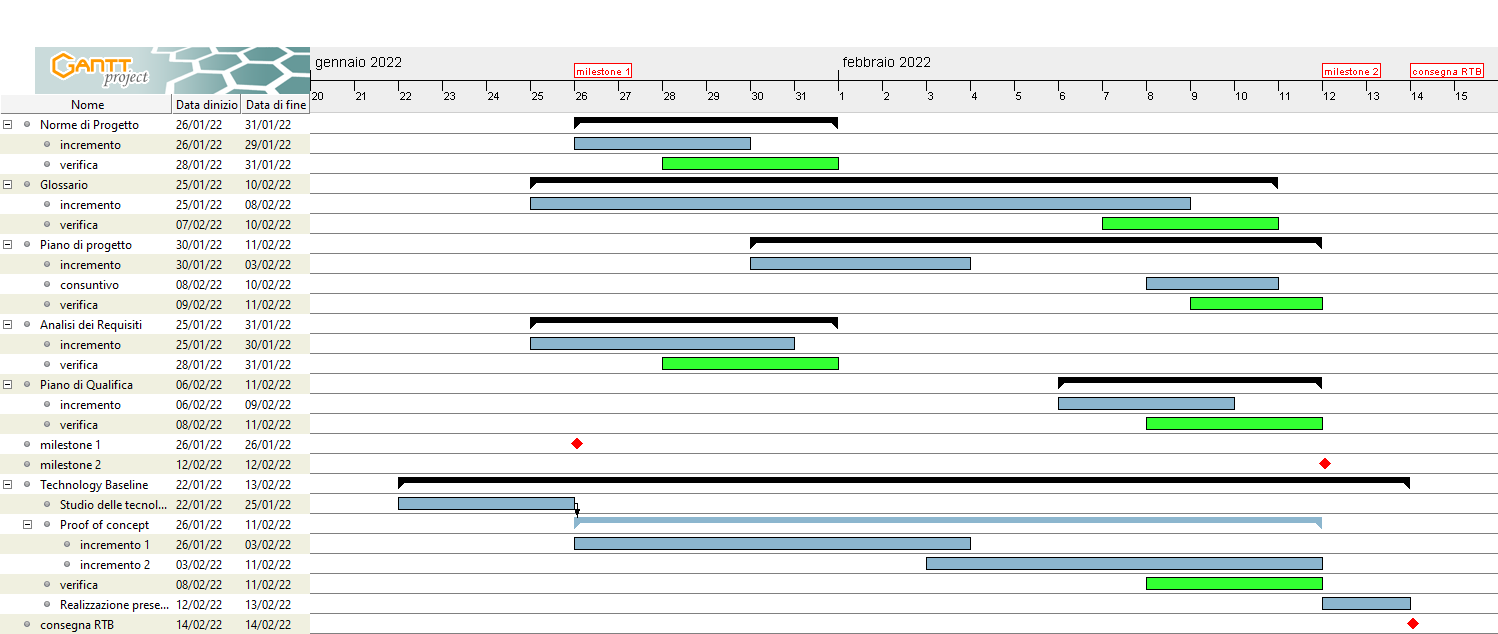
\includegraphics[scale=0.25]{Sezioni/gantt/TB.png}
    \caption{Diagramma di Gantt - Produzione del Proof of Concept}
\end{figure}